\documentclass{article}
\usepackage{graphicx} % Required for inserting images
\graphicspath{{Images/}}
\usepackage[utf8]{inputenc}
\usepackage{multicol}
\usepackage{amsthm}
\usepackage{amsmath}
\usepackage{xcolor}

\newtheorem{definition}{Definition}[section]
\newtheorem{remark}{Remarque}[section]
\newtheorem{theorem}{Théorème}

\title{Analyse I}
\author{Laura Paraboschi / Simon Lefort }
\date{BA1 - IN}

\begin{document}

\maketitle

\section{Règles de calcul}

\begin{multicols}{2}
\subsection{Puissance}  
\columnbreak
\subsection{Logarithme}
\end{multicols}

\begin{multicols}{2}

\begin{itemize}
    \item \( a^n \cdot a^m = a^{m+n} \)
    \item \( (ab)^m = a^mb^m \)
    \item \( (\frac{a}{b})^m = (\frac{a^m}{b^m}) \)
    \item \( \frac{a^m}{a^n} = a^{m-n} \)
\end{itemize}
\columnbreak

\begin{itemize}
    \item \( \log_a(x \cdot y) = \log_a(x) + \log_a(y) \)
    \item \( \log_a(\frac{1}{x}) = -\log_a(x) \)
    \item \( \log_a(\frac{x}{y}) = \log_a(x) - \log_a(y) \)
    \item \( \log_a(x^r) = r\log_a(x) \)
\end{itemize}

\end{multicols}

\section{Ensemble}
\begin{definition}
P(X) est l'ensemble dont les éléments sont tous les sous-ensembles de X. Sa capacité est de  \(2^n\), avec n = nombres d'élements dans X
\end{definition}
\subsection{Produit cartésien}
\[ X \times Y \times Z := \{\,(x,y,z)\quad |\quad x \in X,\,y \in Y,\, z \in Z\, \} \]
\begin{definition}
    Un sous ensemble \(R \subset X \times Y\) est appelé \underline{une relation binaire} sur X et Y
\end{definition}
\begin{definition}
    Un sous ensemble \(R \subset X \times X\) est appelé \underline{une relation} sur X
\end{definition}

\subsection{Classe d'équivalence}
\begin{definition}
    Un sous ensemble \(R \subset X \times X\) est appelé \underline{une relation d'équivalence} sur X si :
    \begin{enumerate}
        \item \( \forall x \in X,\quad x \sim x \) (R est réflexive)
        \item \( \forall x,\,y \in X,\quad  x \sim y \Rightarrow y \sim x \) (R est symétrique)
        \item \( \forall x,\,y,\, z \in X,\quad x \sim y\, \wedge\, y \sim z \Rightarrow x \sim z \) (R est transitive)
    \end{enumerate}
\end{definition}
\begin{definition}
    On définit \(C_x \subset X \) par \\ \[ C_x := \{\, y \in X\quad |\quad y \sim x\, \} \] \\
    \(C_x\) est appelé la classe d'équivalence de x
\end{definition}
\begin{definition}
    L'ensemble quotient \(X/_\sim \) est l'ensemble des classes d'équivalences distinctes de X
\end{definition}
\subsection{Fonction}
\begin{definition}
    Une fonction f : \(D \rightarrow Y\) est appelée 
    \begin{itemize}
        \item \underline{surjective} si Im(f) = Y
        \item \underline{injective} si \( f(x_1) = f(x_2) \Rightarrow x_1 = x_2 \)
    \end{itemize}
\end{definition}
\begin{remark}
    \( (A \Rightarrow B) \Leftrightarrow (\overline{A} \Rightarrow \overline{B}) \) \quad Une proposition contraposée
\end{remark}
\begin{remark}
    Toute fonction f : \(D \rightarrow Y\) définit une fonction surjective\\ \[f : D \rightarrow Im(f) \subset Y\]
\end{remark}
\begin{definition}
    Une fonction qui est surjective et injective est appelée bijective
\end{definition}
\begin{remark}
    Toute fonction bijective \(D \rightarrow Y\) possède une fonction réciproque notée \( f^{-1}, Y \rightarrow D\)
\end{remark}
Soient deux fonctions f :\(D \rightarrow Y\) et g : \(E \rightarrow Y\) avec \(E \subset D\), telle que pour tout \(x \in E, g(x) = f(x)\). Alors :
\begin{itemize}
    \item g est appelée la restriction de f à E : \(g = f|_E\)
    \item f est appelée un prolongement de g de E à D
\end{itemize}
\begin{definition}
    Le graphe d'une fonction f : \(D \rightarrow Y\) est l'ensemble
    \[ G_f := \{\, (x,y) \in D \times Y\quad |\quad y = f(x)\, \} \]
    \qquad Attention, pour tout x, il ne doit exister \textcolor{red}{qu'une seule} image (qu'un seul y = f(x)).
\end{definition}
\begin{definition}
    On définit \(h = g \circ f\) comme étant la composition de fonction 
    \[h = g(f(x))\]
    \qquad La loi de la composition de fonction est associative
\end{definition}
\newpage
\section{Plus grand commun diviseur}
\subsection{Algorithme de J. Stein}
\begin{itemize}
    \item pgcd(a,b) = pgcd(b,a)
    \item pgcd(a,b) = 2\(\cdot\) pgcd(\(\frac{a}{2},\frac{b}{2})\) \qquad si a, b pairs
    \item pgcd(a,b) = pgcd(\(\frac{a}{2}\),b) \qquad si a pair, b impair
    \item  pgcd(a,b) = pgcd(\(\frac{a-b}{2}\), b)  \qquad si a, b impairs et a \(\geq \) b
    \item pgcd(a,0) = a
\end{itemize}
\section{Raisonnement par récurrence}
\begin{theorem} 
\end{theorem}
\begin{enumerate} 
    \item Si P(\(n_0)\) est vrai pour un \(n_0 \in \mathbf{N}\)
    \item Si pour tout n \(\geq n_0\), P(n) \(\Rightarrow\) P(n+1)
\end{enumerate}
\qquad \textit{Alors P(n) est vrai pour tout n \(\geq n_0\)}
\section{Les notations \(\Sigma\) et \(\Pi\)}
\(\sum_{k=m}^n a_k := a_m + a_{m+1} + ... + a_{n-1} + a_n \) \\\\
\( \prod_{k=m}^{m} a_k := a_m \cdot a_{m+1} \cdot ... \cdot a_{n-1} \cdot a_n\)\\\\
\( Si\ n < m, alors \qquad \sum_{k=m}^{n} a_k := 0,\qquad \prod_{k=m}^{n} a_k = 1 \)
\subsection{Règles de calcul}
\( \sum_{k=l}^{m} a_k + \sum_{k=m+1}^{n} a_k = \sum_{k=l}^{n} a_k \)\\\\
\( (\prod_{k=l}^{m} a_k)\cdot(\prod_{k=m+1}^{n} a_k) =\prod_{k=l}^{n} a_k \)\\\\
\( \sum_{k=m}^{n}(a_k + b_k) = \sum_{k=m}^{n} a_k + \sum_{k=m}^{n} b_k \)\\\\
\( \prod_{k=m}^{n}(a_k \cdot b_k) = (\prod_{k=m}^{n} a_k) \cdot (\prod_{k=m}^{n} b_k)\)
\subsection{Identité}
\(\sum_{k=0}^{n} a^k = \frac{1-a^{n+1}}{1-a}, \qquad a \neq 1\)\\\\
\( \sum_{k=0}^{n} k = \frac{n\cdot(n+1)}{2} \)\\\\
\( (a + b)^2 = a^2 + 2ab + b^2  \)\\\\
\( (a + b)^3 = a^3 + 3a^2b + 3ab^2 + b^3 \)\\\\
\( (a + b)^n = \sum_{k=0}^{n} 
\begin{pmatrix}
    n \\ k
\end{pmatrix} a^{n-k}\cdot b^k = a^n + na^{n-1}b + ... + b^n \)\\\\
On peut tout déduire du triangle de Pascal :
\begin{figure}[htp]
    \centering
    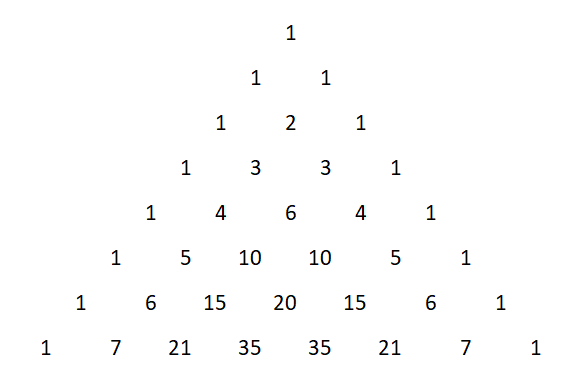
\includegraphics[width=8cm]{Images/Pascal-Triangle.png}
    \caption{Triangle de Pascal}
\end{figure}
\section{Nombres réels}
\begin{definition}
Un corps est un ensemble muni des opérations + et $ \cdot $, rendant possible le calcul d'opposés et d'inverses
\end{definition}
\begin{definition}
    R est un corps qui a les propriétés suivantes :
    \begin{multicols}{2}
        
    
    \begin{itemize}
        \item x + (y + z) = (x + y) + z
        \item x + y = y + x
        \item 0 + x = x
        \item (-x) + x = 0 
        \columnbreak
        \item \( x \cdot (y \cdot z) =  (x \cdot y) \cdot z\)
        \item \( x \cdot y = y \cdot x\) 
        \item  \(1 \cdot x = x \)
        \item \( x^{-1} \cdot x = 1\)
        \item \(x \cdot (y + z) = x \cdot y + x \cdot z\)
    \end{itemize}
    \end{multicols}
    Un corps \underline{ordonné} est en plus compatible avec \( \leq \) 
\end{definition}
\begin{definition}
    Un corps archimédien a la propriété suivante :\\
    Pour tout x, y \(\in\) au corps, x \(>\) 0, y \(\geq\) 0 il existe n \(\in N^*\) tel que nx \(>\) y
\end{definition}
Les démonstrations peuvent être faites de plusieurs manières différentes :
\begin{itemize}
    \item Raisonnement déductif : Si A est vrai et A \(\implies\) B, alors B est vrai
    \item Raisonnement par l'absurde : Si B est vrai et A \(\implies \overline{B}\), alors \(\overline{A}\) est vrai
\end{itemize}
\subsection{Infimum et Supremum}
\underline{minimum} : plus petite valeur de A \\
\underline{maximum} : plus grande valeur de A \\
\underline{minorant} : a \(\leq\) x, a appartenant à R, x appartenant à A \\ infimum (ou borne inférieure) si a est le plus grand minorant \\\\
\underline{majorant} : x \(\leq\) a, a appartenant à R, x appartenant à A  \\ suprémum (ou borne supérieure) si a est le plus petit majorant\\\\
\underline{minoré} : A admet un minorant \\
\underline{majoré} : A admet un majorant \\
\underline{borné} : A admet un minorant et un majorant
\begin{remark}
    Un majorant/minorant peut être un maximum/minimum s'il appartient à A
\end{remark}
\subsection{Valeur absolue}
Inégalités triangulaires :
\begin{itemize}
    \item \( |x \pm y| \leq |x| + |y| \)
    \item \( |x \pm y| \geq ||x| - |y|| \)
\end{itemize}
Identités :
\begin{itemize}
    \item \( |x +\ y| + |x -\ y| =  |x| + |y| + ||x| - |y|| = 2 \cdot max\{|x|, |y|\}\)
    \item \( |x +\ y| - |x -\ y|| =  |x| + |y| - ||x| - |y|| = 2 \cdot min\{|x|, |y|\}\)
\end{itemize}
\section{Nombres complexes}
\begin{definition}
   \( \mathbf{C} = (X, +, \cdot) \qquad X = \mathbf{R} \times \mathbf{R} \)\\\\
   \( + : (a, b) + (c, d) = (a + c,\ b + d)\) \\\\
   \( \cdot : (a, b) \cdot (c, d) = (ac - bd,\ ad + bc) \)
\end{definition} \newpage
\subsection{Représentation cartésienne}
\begin{figure}[htp]
    \centering
    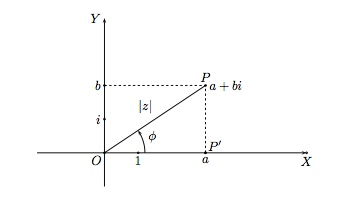
\includegraphics[width=12cm]{Images/complexe2.jpeg}
    \caption{Représentation des nombres complexes}
    \label{fig:complex}
\end{figure} 
\underline{Notations :} 
\begin{itemize}
    \item i = (0,1) et \(i^2\)= -1 (-1, 0), c'est l'unité imaginaire 
    \item z = a + ib, \qquad \qquad \qquad \qquad avec a = Re(z) = \( \frac{z + \overline{z}}{2}\) et b = Im(z) = \( \frac{z - \overline{z}}{2}\)
\end{itemize}
\subsection{Définitions additionelles}
\begin{figure}[htp]
    \centering
    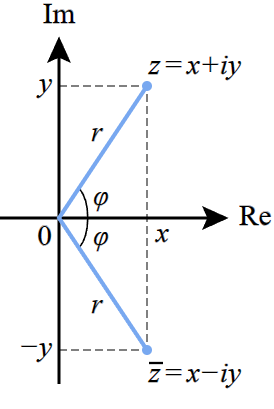
\includegraphics[height=4cm]{Images/conjugue.png}
    \label{fig:conjugue}
\end{figure}
Le \underline{complexe conjugué} de z : \( \overline{z} = a - ib\) \\
\begin{itemize}
    \item \( \overline{\overline{z}} = z \)
    \item \( \overline{z_1 + z_2} = \overline{z}_1+ \overline{z}_2 \)
    \item \( \overline{z_1 \cdot z_2} = \overline{z}_1 \cdot \overline{z}_2 \)
\end{itemize} \newpage
Le \underline{module} de z : \(|z| = (z\cdot\overline{z})^{\frac{1}{2}} = \sqrt{z\cdot\overline{z}} = \sqrt{a^2 + b^2} = |\overline{z}|\)
\begin{itemize}
    \item \( |z_1 \cdot z_2| = |z_1|\cdot|z_2| \)
\end{itemize}
L'\underline{élément inverse} de z : \(\frac{1}{z} = \frac{1}{|z|^2}\cdot\overline{z}\)
\begin{itemize}
    \item \(Re(\frac{1}{z}) = \frac{a}{a^2 + b^2}, \ Im(\frac{1}{z}) = \frac{-b}{a^2 + b^2} \)
    \item \( \frac{z_1}{z_2} = z_1 \cdot \frac{1}{z_2} \)
\end{itemize}
\underline{Formule d'Euler}
\[ e^{i\phi} = \cos{\phi} + i\sin{\phi} \]
\[ e^{z_1} \cdot e^{z_2} = e^{z_1 + z_2} \]
\[ \overline{e^z} = e^{\overline{z}} \]
\[ (e^z)^n = e^{n\cdot z} \]
\underline{Formule de Moivre}
\[ \cos{n\phi} + i\sin{n\phi} = (\cos{\phi} + i\sin{\phi})^n \]
\begin{itemize}
    \item \( \cos{\phi} = \frac{e^{i\phi} + e^{-i\phi}}{2} \Rightarrow \cos{z} = \frac{e^{iz} + e^{-iz}}{2} \)
    \item \( \sin{\phi} = \frac{e^{i\phi} - e^{-i\phi}}{2} \Rightarrow \sin{z} = \frac{e^{iz} - e^{-iz}}{2} \)
\end{itemize}
\underline{Forme polaire} : z = \( |z|\cdot e^{i\phi} \) \qquad \qquad \qquad \( \phi \in [0, \pi]\)
\begin{itemize}
    \item arg(z) = \(\phi\) = 2 \( \arctan{\frac{b}{a + |z|}} \) ou \( \arctan{\frac{b}{a}}\) si a $>$ 0 (ou vérifier le cadran)
    \item \( z_1z_2 = |z_1||z_2|e^{i(\phi_1 + \phi_2)} \)
    \item \( \frac{1}{z} = \frac{1}{r}e^{-i\phi} \)
\end{itemize}
\subsection{Résolution d'équations}
\underline{Racines n-ièmes :}
\[ z^n = w\]
\[ \Leftrightarrow {(re^{i\theta})}^n = w\]
\[ \Leftrightarrow r^n \cdot e^{in\theta} = w\]
\[ \Leftrightarrow p \cdot e^{i(\lambda + 2k\pi)} = w\]

On en déduit :
\[ r^n = p \]
\[ n\theta = \lambda + 2k\pi, k \in \mathbf{Z} \]
Méthode polaire :
\begin{enumerate}
    \item \( w = |w|e^{i(\phi + 2k\pi)} \) \qquad \qquad \qquad k = 0, ..., n-1
    \item \( z_{k+1} = |w|^{\frac{1}{n}}e^{i(\frac{\phi}{n} + 2\frac{k}{n}\pi)} \) \qquad \qquad \qquad k = 0, ..., n-1
\end{enumerate}
Méthode cartésienne :
\[ z^n = a + ib \]
On cherche Re(z) = Re(w) \underline{et} Im(z) = Im(w) \\
\textcolor{red}{Attention aux solutions éventuelles qui pourraient apparaître et ne sont pas solutions de l'équation de base}
\\\\
\underline{Théorème fondamental de l'algèbre :} \\\\
Tout polynôme p(z) = \( a_nz^n+...+a_1z +a_0 \) admet dans les complexes n racines, on peut donc l'écrire :
\[ p(z) = a_n(z - z_1)(z - z_2)...(z - z_n)\]
\begin{remark}
    Si \(p(z_k) = 0\) alors \(p(\overline{z_k}) = 0\) donc les racines sont soit des nombres réels soit des paires de nombres complexes conjugués \textcolor{red}{Attention, seulement pour des coefficients réels !}
\end{remark}
\(\Rightarrow\) Tout polynôme à coefficients réels peut être factorisé dans R en facteurs linéaires et quadratiques
\begin{remark}
    \( z^2 - az + b = z^2 - 2Re(z_k)z + |z_k|^2 = (z - z_k)(z - \overline{z_k})\)
\end{remark}
\underline{Formule de Viète}
\[ z_{1,2} = \frac{-b \pm \sqrt{\Delta}}{2a} \quad avec \quad \Delta = b^2 - 4ac \geq 0\]
\[ z_{1,2} = \frac{-b \pm i\sqrt{-\Delta}}{2a} \quad avec \quad \Delta = b^2 - 4ac < 0\]

\begin{remark}
Simplification des exposants de i
    \[ i^{4k} = 1 \]
    \[ i^{4k+1} = i \]
    \[ i^{4k+2} = -1 \] 
    \[ i^{4k+3} = -i \]
\end{remark}
\begin{remark}
Propriétés importantes des logarithmes
    \[ ln(a^{b}) = bln(a) \]
    \[ e^{ln(a^{b}}) = a^{b} \]
    \[ \Rightarrow e^{bln(a)} = a^{b} \]
\end{remark}

\section{Suites de nombres réels}

\begin{definition}
Une suite est une fonction qui associe un entier naturel à un réel. \\
    $ f : \mathbf{N} \rightarrow \mathbf{R} $ \\
    $ f : n \rightarrow f(n) = a_n $
\end{definition}

\subsection{Limite de suite}

La suite $ a_n $ est convergente s'il existe un $ a \in \mathbf{R} $ tel que : \\
\[ \forall \epsilon > 0,\ \exists n_0 \in \mathbf{N},\ \forall n > n_0,\ |a_n - a| < \epsilon \]\\
divergente $ \Leftrightarrow $ non-convergente\\
oscille $ \implies $ divergente \\
Toute suite convergente est bornée!

\subsubsection{Limite vers + ou - infini}

Une suite divergente tend vers + ou - l'infini si :

\[ \forall r \in \mathbf{R}, \exists n_0, \forall n \geq n_0, |a_n|  \geq r \]

\subsubsection{Unicité de la limite}
Voir théoremes

\subsubsection{Définition de inf et sup}

\textbf{inf(A)}\\
\[ \forall \epsilon > 0,\ \exists n_0 \in \mathbf{N}\ \text{t. q.}\ a_{n_0} < inf(A) + \epsilon \]
\textbf{sup(A)}\\
\[ \forall \epsilon > 0,\ \exists n_0 \in \mathbf{N}\ \text{t. q.}\ a_{n_0} > sup(A) - \epsilon \]
Remarque, si supA appartient à la suite alors c'est le max de la suite, min pour le inf.

\subsection{Operations algébriques sur les limites}
\underline{Si lim(an) = a et lim(bn) = b, alors}\\
\begin{itemize}
    \item lim($\alpha a_n + \beta b_n$) = $\alpha lim(a_n) + \beta lim(b_n)$
    \item lim($a_n \cdot b_n)$ = lim($a_n$) $\cdot$ lim($b_n)$
    \item lim($\frac{a_n}{b_n}$) = $\frac{lima_n}{limb_n}$ = $\frac{a}{b}$ si b $\neq$ 0
\end{itemize}
\subsubsection{Théorème des gendarmes}

\textbf{Hypothèses} \\
\[ \lim_{n\to\infty}a_n = \lim_{n\to\infty}b_n = c \]
\[ a_n < C_n < b_n\ \forall n \geq m \]
\textbf{Alors} \\

\[ \forall \epsilon > 0,\ \exists n_0 \geq m\ \text{t.q.}\ \forall n \geq n_0\ \text{:} \]
\[ \lvert a_n - c \lvert < \epsilon \]
\[ \lvert b_n - c \lvert < \epsilon \] \\\\
Notes :\\\\
voir Theorems
\subsection{Convergence d'une suite définie par récurrence}
Montrée que la suite est minoréee + décroissamte ou majorée + croissante
(1. Calculer lim, 2. minorée/majorée, 3. croissante/décroissante)

\subsubsection{Théorème de d'Alembert}

Soit $ q = \lim_{n\to\infty}\ \lvert \frac{a_{n+1}}{a_n} \lvert $.\\
\begin{itemize}
    \item Si $ 0 \leq q < 1 $, la suite $ a_n $ converge vers 0.
    \item Si $ q = 1 $, on ne sait pas.
    \item Si $ q > 1 $, la suite $ a_n $ diverge.
\end{itemize}

\subsubsection{Suites de Cauchy}

Une suite est appelée suite de Cauchy si :\\
\[ \forall \epsilon > 0,\ \exists N\ \in \mathbf{N},\ \forall n,\ m \geq N,\ |a_n - a_m| < \epsilon \]

Dans R toutes les suites de Cauchy sont convergentes mais pas dans les espaces non complets (ex. Q). "ça converge vers quelque chose qui n'existe pas", donc $ \neg\exists{a} $, avec $ a $ la limite.

\subsubsection{Sous-suites}
On a une fonction g qui fait un remapping des index en en supprimant certains par ex., mais en gardant un ordre croissant.

\[ f : \mathbf{N} \rightarrow \mathbf{R}\ \mathrm{(suite\ a_n)} \]
\[ g : \mathbf{N} \rightarrow \mathbf{N}\ \mathrm{(strictement\ croissante)} \]
\[ \mathrm{composition :\\} \mathbf{N} \xrightarrow{g} \mathbf{N} \xrightarrow{f} \mathbf{R} \]

\paragraph{Convergence des suites définies par récurrence}
$ \newline \newline $
Si une suite $ a_n = g(a_{n-1} $ avec $ g(x) = q \cdot x + b $, alors :\\\\
Soit $ a = \frac{b}{1 - q}$
\begin{itemize}
    \item Si $ |q| < 1 $, la suite converge vers $ a $.
    \item Si $ |q| > 1 $, la suite diverge.
\end{itemize}
\begin{remark}
    On peut trouver a en posant a = g(a)
\end{remark}
\subsection{Théorème de Bolzano-Weierstrass}
De toute suite $a_n$ bornée, on peut extraie une sous suite convergente \\\\
a $\in$ R est un point d'accumulation d'une suite $a_n$ s'il existe une sous-suite $d_k$ telle que $\lim_{k\to\infty}d_k = a \implies$  Toute suite bornée à au moins un point d'accumulation

\subsection{Limite inférieure et supérieure}
La limite inférieure est le plus petit des points d'accumulation \\\\
La limite supérieure est le plus grand des points d'accumulation
\begin{remark}
    $\liminf_{n\to\infty}a_n = \limsup_{n\to\infty}a_n = a \Leftrightarrow \lim_{n\to\infty}a_n = a$
\end{remark}

\section{Séries numériques}

Soit $ a_n $ la suite des termes d'une série. \\
$\sum_{k=0}^{\infty}a_k = \lim_{n\to\infty}s_n, s_n = \sum_{k=0}^{n}a_k$ (somme partielle) \\\\
La limite s de $s_n$ est appelée la somme de la série numérique \\\\
Une série $\sum_{k=0}^{\infty}a_k $ est dite absolument convergente si $\sum_{k=0}^{\infty}|a_k| $ converge
\subsection{Critères de convergence}

\subsection{Exemples}

Série harmonique $ \sum \frac{1}{k} $ diverge.\\\\
Série harmonique alternée $ \sum (-1)^{(k-1)} \cdot \frac{1}{k} $ converge (mais pas absolument).\\\\
Série géométrique $\sum q^k $ converge absolument pour $ |q| < 1 $ et diverge sinon.

\subsection{Critère nécéssaire}
$\sum_{k=0}^{\infty}a_k$ converge $\implies \lim_{k\to\infty}a_k = 0$ (voir theorems)
\subsubsection{Critère de d'Alembert}

On pose $ q = \lim_{n\to\infty}\ \lvert \frac{a_{n+1}}{a_n} \lvert $.\\\\
Si $ 0 \leq q < 1 $, alors la série converge absolument.\\
Si $ q = 1 $, on ne sait pas.\\
Si $ q > 1 $, la série diverge.

\subsubsection{Critère de Cauchy}

On pose $ q = \lim_{n\to\infty}\ {\lvert a_{n}\lvert}^{1/n} $.\\\\
Si $ 0 \leq q < 1 $, alors la série converge absolument.\\
Si $ q = 1 $, on ne sait pas.\\
Si $ q > 1 $, la série diverge.

\subsubsection{Critère du limsup}

On pose $ q = \limsup_{n\to\infty}\ {\lvert a_{n}\lvert}^{1/n} $.\\\\
Si $ 0 \leq q < 1 $, alors la série convereg absolument.\\
Si $ q = 1 $, on ne sait pas.\\
Si $ q > 1 $, la série diverge.

\subsubsection{Convergence des séries alternées (Leibniz)}

Les séries alternées associées $ \sum_{k=1}^{\infty} (-1)^k \cdot a_k $ convergent absolument si :
\begin{itemize}
    \item La suite $ |a_k| $ est strictement décroissante.
    \item $ \lim_{n\to\infty} a_k = 0 $
\end{itemize}

\subsubsection{Critère de comparaison 1}

\begin{itemize}
    \item $ \forall\ k,\ 0 \leq \lvert a_k \lvert\ \leq b_k $
    \item $ \sum_{k=1}^{\infty} b_k $ converge
\end{itemize}

$ \implies \sum_{k=1}^{\infty} a_k $ converge absolument.

\subsubsection{Critère de comparaison 2}

\begin{remark}
    Généralement on essaye de minorer la suite par la suite harmonique, dont la série diverge.
\end{remark}

\begin{itemize}
    \item $ \forall\ k,\ 0 \leq b_k \leq a_k $
    \item $ \sum_{k=1}^{\infty} b_k $ diverge
\end{itemize}

$ \implies \sum_{k=1}^{\infty} a_k $ diverge.

\section{Fonctions réelles}
\subsection{Types de fonctions}
\begin{itemize}
    \item Polynôme : $ \sum_{k = 0}^{n}a_kx^k $
    \item Rationnelle : $ \frac{p(x)}{q(x)} $
    \item Algébrique : Fonctions polynômes et un nombre fini d'opérations
    \item Transcendante : Fonctions non algébriques $e^x.\ ln(x),\ sin(x)$
\end{itemize}
Croissance et décroissance :
\begin{itemize}
    \item une fonction est croissante si : $ x_1 \leq x_2 \implies f(x_1) \leq f(x_2) $
    \item une fonction est décroissante si : $ x_1 \leq x_2 \implies f(x_1) \geq f(x_2) $
\end{itemize}
\begin{theorem}
    Une fonction strictement monotone est injective.
\end{theorem}

\begin{definition}
    Un ensemble $ X \subseteq R $ est symmétrique si $ \forall x, (x \in X \implies -x \in X) $.
\end{definition}

\subsection{Fonctions paires et impaires}
\begin{definition}
    Une fonction est paire si son ensemble de définition est symmétrique \textbf{et} $ \forall x \in D, (f(x) = f(-x)).$
\end{definition}
\begin{definition}
    Une fonction est impaire si son ensemble de définition est symmétrique \textbf{et} $ \forall x \in D, (f(x) = -f(-x)).$
\end{definition}

\begin{definition}
    Une fonction est périodique de période $ T > 0 $ si $ \forall x \in D, (f(x+T) = f(x)) $. Le plus petit $ T $ qui satisfait la définition est appelé la période de f. Remarque: implique $ \forall x \in D, \forall n \in \mathbf{Z}, x + nT \in D$. 
\end{definition}

Toute fonction dont le domaine de définition est symmétrique peut être décomposée en une somme d'une fonction paire et d'une fonction impaire.

\[ f(x) = f(x) + \frac{1}{2} f(-x) - \frac{1}{2} f(-x) \]
\[ \Leftrightarrow f(x) = \frac{1}{2}(f(x) + f(-x)) + \frac{1}{2}(f(x) - f(-x)) \]
\[ \Leftrightarrow f(x) = f_{+}(x) + f_{-}(x) \]

\subsubsection{Cosh et Sinh}

\[ cosh(x) = \frac{e^x + e^{-x}}{2} \hspace{0.3cm} \text{(paire)} \]
\[ sinh(x) = \frac{e^x - e^{-x}}{2} \hspace{0.3cm} \text{(impaire)}\]

\[ f(x) = e^x = cosh(x) + sinh(x) \]
\begin{remark}
    \[ cosh^2(x) - sinh^2(x) = 1 \]
\end{remark}

\subsubsection{Identités}

Soit $ p_1, p_2 $ des fonctions paires.\\
Soit $ i_1, i_2 $ des fonctions impaires.

\begin{itemize}
    \item $ p_1 + p_2 $ est \textbf{paire}
    \item $ p_1 \cdot p_2 $ est \textbf{paire}
    \item $ i_1 + i_2 $ est \textbf{impaire}
    \item $ i_1 \cdot i_2 $ est \textbf{paire}
    \item $ p_1 \cdot i_1 $ est \textbf{impaire}
    \item $ p_1 \circ i_1 $ est \textbf{paire}
    \item $ f \circ p_1 $ est \textbf{paire}
    \item $ i_1 \circ i_2 $ est \textbf{impaire}
\end{itemize}
Soient f et g des fonctions périodiques de période $ T_f $ et $ T_g $.\\\\
On a $ h\circ f$, $ T_f $-périodique (mais ce n'est pas la période (le plus petit T)!).\\\\
De plus, $ \frac{T_f}{T_g} \in \mathbf{Q} \implies $

\begin{itemize}
    \item $ f + g $ est périodique
    \item $ f \cdot g $ est périodique
\end{itemize}
$\frac{T_f}{T_g} = \frac{p}{q} \implies T = p \cdot T_g = q \cdot T_f$ (pas la période)
\subsection{Inverse et préimage}

\subsubsection{Inverse}

Si f est bijective alors $ f^{-1} $ dénote l'inverse où $ f(f^{-1}(x)) = x = f^{-1}f((x))$
\subsubsection{Préimage}

f n'a pas besoin d'être bijective\\
$ f^{-1}(\{y\}) = \{ x \in D_f | f(x) = y\}$\\
Si f est bij. alors $ f^{-1}(\{y\}) = \{f^{-1}(y)\} $

\subsection{Fonctions définies par étape}
Faire chaque cas possible \\\\
signum:
\begin{equation}
sign(x)=
    \begin{cases}
        1 & \text{if } x > 0\\
        0 & \text{if } < = 0\\
        -1 & \text{if } x < 0
    \end{cases}
\end{equation}
heaviside:
\begin{equation}
H(x)=
    \begin{cases}
        1 & \text{if } x > 0\\
        0 & \text{if } x \leq 0
    \end{cases}
\end{equation}

\subsection{Transformations affines}

\[ g(x) = f(ax + b) \]
\textbf{translation (b)}
\begin{itemize}
    \item $ b > 0 $, le graphe est décalé vers la gauche
    \item $ b < 0 $, le graphe est décalé vers la droite
\end{itemize}
\textbf{compression/dilatation/réflexion (a)}
\begin{itemize}
    \item $ |a| > 1 $, le graphe est comprimé
    \item $ 0 < |a| < 1 $, le graphe est dilaté
    \item $ a < 0 $, le graphe est inversé horizontalement (par rapport à l'axe des ordonnées)
\end{itemize}

\paragraph{intuition/exemples}
si on pose $ f(x) = x $ et $ g(x) = x - 4 $, pour retrouver l'origine 0, on doit aller à x = 4, donc on se décale vers la droite.\\
si on pose $ g(x) = 2x $, on va comprimer le graphe (ici faire monter la courbe plus vite).

\subsection{Limite (épointée) d'une fonction}

$ f : D \to \mathbf{R} $ admet pour limite épointée $ l \in \mathbf{R} $ lorsque $ x \to x^* $ si $ \forall (x_n) $ t.q $ \forall n, x_n \in D \backslash \{x^*\} $ t.q $ \lim_{n\to\infty} x_n = x^*$, la suite $ y_n = f(x_n) $ converge et $ \lim_{n\to\infty} y_n = l$\\\\
La valeur de $ f(x^*) $ peut être différente de la valeur de la limite en $ x^* $.\\\\
\textit{voir dans les théorèmes 5/6 pour des exemples}

\subsubsection{Définition équivalente}

$ f : D \to \mathbf{R} $ admet pour limite épointée $ l \in \mathbf{R} $ lorsque $ x \to x^* $ si $ \forall \epsilon > 0, \exists \delta > 0, \forall x \in D, (0 < |x-x^*| \leq \delta) \implies |f(x) - l| \leq \epsilon)$

\subsubsection{Limite (épointée) à gauche ou à droite}

On modifie la définition du haut en rajoutant pour condition soit que $ \forall x_n (x_n < x^*) $ (si on veut la limite à gauche), soit $ \forall x_n (x_n > x^*)$ si on veut la limite à gauche et on introduit les notations $ l_+ $ et $ l_-$.

\subsection{Opérations algébriques sur les limites}

Ici la limite correspond à la limite épointée, la limite à gauche ou la limite droite. On doit garder le même choix pour toutes les implications.

\[ (lim_{x\to{x^*}} f(x) = a \wedge \lim_{x\to{x^*}} g(x) = b) \]
\[ \implies \]
\[ (lim_{x\to{x^*}} (f(x) + g(x)) = \lim_{x\to{x^*}} f(x) + \lim_{x\to{x^*}} g(x) = a + b) \]
\[ \wedge\ (lim_{x\to{x^*}} (f(x) \cdot g(x)) = \lim_{x\to{x^*}} f(x) \cdot \lim_{x\to{x^*}} g(x) = a \cdot b) \]
\[ \wedge\ (b \neq 0 \implies \lim_{x\to{x^*}} \frac{f(x)}{g(x)} = \frac{lim_{x\to{x^*}} f(x)}{lim_{x\to{x^*}} g(x)} = \frac{a}{b}) \]

\subsection{Limites + ou - l'infini}

\subsubsection{Limite égale à l'infini en un point}

\[ \lim_{x\to{x^*}} f(x) = +\infty \in \mathbf{R} \]
\[ \Leftrightarrow \]
$ \forall $ suite $ (x_n), x_n \in D(f) $ et $ \lim_{n\to\infty} x_n = x^* $, on a: $ \lim_{n\to\infty} f(x_n) = +\infty $

\subsubsection{Limite évaluée à l'infini}

\[ \lim_{x\to\infty} f(x) = l \in \mathbf{R} \]
\[ \Leftrightarrow \]
$ \forall $ suite $ (x_n), x_n \in D(f) $ et $ \lim_{n\to\infty} x_n = +\infty $, on a: $ \lim_{n\to\infty} f(x_n) = l $

\subsection{Limites et composition de fonction}

Soit $ f, g : \mathbf{R} \to \mathbf{R} $ et $ h = g \circ f $\\\\
Si $ \lim_{x\to\infty} f(x) = y^*$ et $ \lim_{\underset{y \neq y^*}{y \rightarrow y^*}} g(y) = l $\\\\
$ \lim_{x\to\infty} g(f(x)) = l $ \textbf{SI} on a bien $ y \neq y^* $ (f doit éviter la valeur de la limite)

\subsection{Fonctions continues en un point}

$ x_0 \in D \subset \mathbf{R}, D \neq \emptyset, $ est appelé un point isolé de $ D $ si $ \exists \epsilon > 0, $ t.q $ ]x_0 - \epsilon, x_0 + \epsilon[\ \cap\ D = \{ x_0 \}$\\\\
Une fonction $ f : D \to \mathbf{R} $ est continue en un point $ x_0 \in \mathbf{D} $ si $ x_0 $ est un point isolé de $ D $ ou si $ \lim_{x\to{x_0}} = f(x_0) $ ("on regarde les deux valeurs à droite et à gauche")\\\\
Remarque : si on sait que $ f $ est continue, on peut calculer la limite en $ x_0 $ en évaluant $ f(x_0) $.

\subsubsection{Définition avec $\epsilon $ et $\delta$}

$ f : D \to \mathbf{R} $ est continue en $ x_0 \in D $ si $ \forall \epsilon > 0, \exists \delta > 0, $ t.q $ \forall \in D, |x - x_0| \leq \delta \implies |f(x) - f(x_0)| \leq \epsilon$

\subsubsection{Fonctions continues}

$ f $ est dite continue ou continue sur $ D $ si $ f $ est continue en tout $ x_0 \in D $.

\subsubsection{Prolongement par continuitié}

Si $ \lim_{x\to{x_0}} f(x) = l \in \mathbf{R} $ mais $ x_0 \notin D(f) $, on définit une fonction $ \hat{f}_{x_0} : D(f) \cup \{x_0\} \to \mathbf{R} $

\begin{equation}
\hat{f}_{x_0}(x) = 
    \begin{cases}
        f(x) & \text{if } x \in D\\
        \lim_{x\to{x_0}}f(x) & \text{if } x = x_0\\
    \end{cases}
\end{equation}
et on a bien $ \hat{f} $ continue.

\subsubsection{Image d'une fonction continue}

L'image $ f(I) $ d'une fonction $f$ continue sur un intervalle $ I = ]a, b[ \subset D$ est un intervalle, mais pas forcément ouvert (tout le temps vrai dans le cas où f est strictement monotone) ni borné.

\subsubsection{Fonctions élémentaires}

La composition de deux fonctions continues est une fonction continue sur son domaine de définition.\\\\
Une \textbf{fonction élementaire} est une fonction construite à partir de fonctions algébriques exponentielles, logarithmiques, sinus et cosinus, et un nombre fini d'opérations $ +, \cdot, /, \circ $.\\\\
Une fonction élementaire est continue sur son domaine de définition.\\\\
Ainsi, pour une fonction élémentaire, $ \forall x_0 \in D, \lim_{x\to{x_0}} f(x) = f(x_0) $

\subsubsection{Fonctions continues sur des intervalles fermés}

Si f est continue sur un intervalle fermé $ D $ si f est continue en tout point $ x \in D $ et aussi à droite et à gauche (quand on a un intervalle fermé on a qu'une seule façon de s'approcher des bornes, par $ a_+ $ (limite à droite) pour la borne inférieure et $ b_- $ (limite à gauche) pour la borne supérieure).

\subsection{Théorème du min max}

Si f est continue, elle admet un minimum et un maximum tq :
\[ f(c) \leq f(x) \leq f(d)\]

\subsection{Méthode de la bissection}
Soit une fonction continue tq g(a) < 0 et g(b) > 0, alors il existe g(c) = 0 et on peut s'en approcher par : \[u_n = \frac{1}{2}(a_n + b_n)\]
\begin{itemize}
    \item $g(u_n) < 0 : a_{n+1} = u_n$
    \item $g(u_n) > 0 : b_{n+1} = b_n $
\end{itemize}

\subsection{Théorème des valeurs intermédiaires}

Soit a, b, toute fonction continue prend (au moins une fois) toutes les valeurs entre f(a) et f(b)

\subsection{Théorème 3}

Soit une fonction continue, alors Imf = [m, M] (minimum et maximum)

\subsection{Théorème du point fixe}

voir fichier theorems.tex

\section{Dérivation}

Soit $ f : D \to \mathbf{R} $ et $ x_0 \in ]a, b[ \subset D \subset \mathbf{R}, a, b \in \mathbf{R}, a < b $.\\\\

\subsection{Dérivabilité}

$ f $ est \textbf{dérivable} en $ x_0 $ si $ f $ admet la limite :
\[ \lim_{x\to{x_0}} \frac{f(x) - f(x_0)}{x - x_0} =: d \in \mathbf{R} \]
\[lim_{h\to{0}} \frac{f{(x_0 + h) - f(x_0)}}{h}\]
c'est à dire, si cette limite existe. On écrit $ d|_{x_0}$ pour se souvenir que c'est la dérivée de $ f $ en $ x_0 $.

\subsection{Différentiabilité}

$ f  $ est différentiable en $ x_0 $ s'il existe un nombre $ \alpha \in \mathbf{R} $ et une fonction reste $ r :\ ]a, b[ \to \mathbf{R} $ tels que $ \forall x \in ]a, b[ $ :
\[ f(x) = f(x_0) + \alpha \cdot (x - x_0) + r(x) \]
\[ f(x_0 + h) = f(x_0) + \alpha \cdot h) + r(x_0 + h) \]  \\\\
avec $ \lim_{x\to{x_0}} \frac{r(x)}{x-{x_0}} = 0 <=>  \lim_{h\to 0} \frac{r(x_0 + h)}{h} = 0 $
\paragraph{Remarque}: $ r(x_0) = 0 $ par définition et $ r(x) $ est dérivable en $ x_0 $ avec pour dérivée 0.

\begin{equation}
\hat{R}(x) = 
    \begin{cases}
         \frac{r(x)}{x-{x_0}} & \text{if } x \in ]a,b[ \setminus {x_o}\\
        0 & \text{if } x = x_0\\
    \end{cases}
\end{equation}
$\implies r(x) = R(x)(x - x_0) $
\subsection{Fonction dérivée}

\[f'(x) = lim_{h\to{0}} \frac{f(x+h) - f(x)}{h}\]

\subsection{Exemple de fonctions dérivées}

$ m \in \mathbf{N^*}$\\
$ p \in \mathbf{R}\ \backslash\ \mathbf{N} $

\begin{center}
\begin{tabular}{||c c c||} 
 \hline
$f$ & $f'$ & $f''$ \\ [0.5ex] 
 \hline\hline
 1 & 0 & 0 \\ 
 \hline
 $x$ & 1 & 0 \\ 
 \hline
 $x^m$ & $m \cdot x^{m-1}$ & \begin{equation}
 \nonumber
 \begin{cases}
    m \cdot (m-1) \cdot ... \cdot (m-n+1) \cdot x^{m-n} & \text{if } n \leq m\\
    0 & \text{if } n > m\\
 \end{cases}
 \end{equation} \\ 
 \hline
 $x^p, (x > 0)$ & $p \cdot x^{p-1}$ & $p \cdot (p-1) \cdot ... \cdot (p-n+1) \cdot x^{p-n}$ \\ 
 \hline
 $sin(x)$ & $cos(x)$ & \begin{equation}
 \nonumber
 \begin{cases}
    (-1)^{n/2} \cdot sin(x) & \text{if} n\ \text{pair} \\
    TODO & \text{if } n > m\\
 \end{cases}
 \end{equation}  \\
 \hline
 $cos(x)$ & $-sin(x)$ TODOO & 0 \\ [1ex] 
 \hline
\end{tabular}
\end{center}
\begin{theorem}
    Une fonction derivable en un point est continue en un point
\end{theorem}
\begin{theorem}
    Une fonction est dérivable en un point si les dérivées à gauche et à droite sont égales
\end{theorem}
\subsection{Opérations algébriques sur les dérivées}
\begin{itemize}
    \item $(\alpha f + \beta g)' =\alpha f' + \beta g' $
    \item $(fg)' = f'g + fg'$
    \item $(\frac{f}{g})' = \frac{f'g - fg'}{g^2}$
\end{itemize}

\subsection{Dérivation en chaîne}

Si f dérivable en $ x_0 $ et g dérivable en $ f(x_0) $ :\\
$(g \circ f)'(x_0) = g'(f(x_0)) \cdot f'(x_0)$

\subsection{Théorème 8.2}

Soit $ f : D \to \mathbf{R} $, $ x_0 \in ]a, b[ $, f continue sur $ ]a, b[ $, dérivable sur $ ]a, b[\ \backslash\ \{x_0\}. $. S'il $ \exists l \in \mathbf{R} $ t.q $ \lim_{x\to{x_0}} f'(x) = l $. Alors $ f $ est dérivable en $ x_0 $ et $ f'(x_0) = l $.
\subsection{Continuité/Dérivabilité de la fonction réciproque}
\begin{theorem}
    La réciproque d'une fonction bijective continue est continue sur l'image de tout intervalle
\end{theorem}
\begin{theorem}
    La réciproque d'une fonction bijective dérivable est dérivable sur l'image de tout intervalle tq f'(x) $\neq$ 0
\end{theorem}
\[(f^{-1})' = \frac{1}{f'(f^{-1}(y))}  \]
\subsection{Théorème de Rolle}
Pour f continuement dérivable\\\\
Si f(a) = 0 et f(b) = 0, alors il existe u tq f'(u) = 0 (u $\in$ [a, b])
\subsection{Théorème des accroissements finis}
Pour f continuement dérivable\\\\
Il existe u tq f'(u) = $\frac{f(b) - f(a)}{b - a}$ (droite parallèle à la droite reliant f(a) et f(b))
\subsection{Implication du TAF}
Réécriture : f(b) = f(a) + f'(u)(b-a) \\\\
Reformulation : $\lambda \in ]0, 1[$ \\
f(x + h) = f(x) + f'(x + $\lambda$ h)h
\subsection{Corollaires du TAF}
\begin{theorem}
    Si f'(x) = 0 sur [a, b] alors f est constante
\end{theorem}
\begin{theorem}   \
\begin{itemize}
    \item f'(x) $\geq$ 0 $\leftrightarrow$ f croissante
    \item f'(x) $>$ 0 $\rightarrow$ f strictement croissante
    \item f'(x) $\leq$ 0 $\leftrightarrow$ f décroissante
    \item f'(x) $<$ 0 $\rightarrow$ f strictement décroissante
\end{itemize}
\end{theorem}
\begin{theorem}
    Si f(a) $\geq$ 0, et f'(x) $\geq$ 0 sur ]a,b[, alors f(x) $\geq$ sur [a,b]
\end{theorem}
\subsection{TAF généralisé} 
$\frac{f'(u)}{g'(u)} = \frac{f(b) - f(a)}{g(b) - g(a)}$
\section{Etudes des fonctions}

\subsection{Bernoulli de l'Hospital}

Soit $ f : D(f) \to \mathbf{R} $ et $ g : D(g) \to {R} $ deux fonctions dérivables sur $ ]a, b[ \subset D(f) \cap D(g), a, b \in \mathbf{R}, a < b $ telles que $ \forall x \in ]a, b[, g'(x) \neq 0 $ et :
\[ \lim_{x\to{a^+}}f(x) = \lim_{x\to{a+}}g(x) = 0\]
\textbf{Si} \[ \lim_{x\to{a^+}}\frac{f'(x)}{g'(x)} = l \in \mathbf{R} \]
\textbf{Alors :}
\[ \lim_{x\to{a^+}}\frac{f(x)}{g(x)} = l \in \mathbf{R} \]
Remarque : généralisation de BH : on a le théorème analogue pour la lim quand x tend vers a- et quand la lim vaut +- infini 

\subsection{Définitions utiles sur graphe}

$ f : I \to \mathbf{R}. I = [a, b], a, b \in \mathbf{R}, a < b $ et $ I_0 \subset I $ est un sous-intervalle fermé.\\

\subsubsection{Convexité}

$ f $ est convexe sur $ I_0 $ si $ \forall x_1, x_2 \in I_0, x_1 < x_2, \forall \lambda \in [0, 1], f(\lambda \cdot x_1 + (1-\lambda) \cdot x_2) $ (la valeur) $ \leq \lambda \cdot f(x_1) + (1-\lambda) \cdot f(x_2)$ (la droite).\\\\
Remarque : si $ \lambda = 1 $ on a $x_1$, si $ \lambda = 0 $ on a $ x_2 $ et sinon on a un point entre $ x_1 et x_2 $, donc l'expression balaie tout l'intervalle $ x_1, x_2$.

\paragraph{Critère} Si $f' $ est croissante sur $ I_0 $ ($f'' \geq 0$) alors $f $ est convexe. Ex : $ x^2 $

\subsubsection{Concavité}

$ f $ est concave sur $ I_0 $ si $ \forall x_1, x_2 \in I_0, x_1 < x_2, \forall \lambda \in [0, 1], f(\lambda \cdot x_1 + (1-\lambda) \cdot x_2) $ (la valeur) $ \geq \lambda \cdot f(x_1) + (1-\lambda) \cdot f(x_2)$ (la droite).\\\\
Remarque : si $ \lambda = 1 $ on a $x_1$, si $ \lambda = 0 $ on a $ x_2 $ et sinon on a un point entre $ x_1 et x_2 $, donc l'expression balaie tout l'intervalle $ x_1, x_2$.

\paragraph{Critère} Si $f' $ est décroissante sur $ I_0 $ ($f'' \leq 0$) alors $f $ est concave. Ex : $ -x^2 $

\subsubsection{Point stationnaire}

$ f $ admet un point stationnaire en $ x_0 \in [a, b] $ si $ f $ est différentiable en $ x_0 $ et $ f'(x_0) = 0$.

\subsubsection{Maximum local}

$ f $ admet un maximum local en $ x_0 \in [a, b] $ si $ f(x) \leq f(x_0) $ pour "$ x $ proche de $ x_0 $". \\
"" $ \Leftrightarrow  \exists \epsilon > 0, $ tel que $ \forall x \in [a,b] $ tel que $ |x-x_0| < \epsilon $.

\subsubsection{Minimum local}

$ f $ admet un minimum local en $ x_0 \in [a, b] $ si $ f(x) \geq f(x_0) $ pour "$ x $ proche de $ x_0 $". \\

\subsubsection{Maximum (ou minimum) global}

$ f $ admet un maximum global en $ x_0 \in [a, b] $ si $ f(x) \leq (\text{ou} \geq) ( f(x_0), \forall x \in [a,b]$.

\subsubsection{Extremum (global ou local)}

$ f $ admet un minimum (global ou local) ou un minimum (global ou local)

\paragraph{Critère} Si $ f $ admet un extremum local en $ x_0 \in ]a, b[$ et si f est dérivable en $ x_0$, alors $ f'(x_0) = 0$.

\begin{itemize}
    \item Si $f'(x_0) = 0$ en $ x_0 \in [a, b]$ et si $ f''(x_0) < 0 $ alors $ f $ admet un maximum local en $ x_0 $.
    \item si $f'(x_0) = 0$ en $ x_0 \in [a, b]$ et $ f''(x_0) > 0$ alors $ f $ admet un minimum local en $ x_0 $.

    \item De façon générale, si $ f'(x_0) = ... = f^{(n)}(x_0) = 0 $, $ f^(n)(x_0) < 0$, n pair $ \Leftrightarrow f $ admet en $ x_0 $ un maximum local.\\
    \item De façon générale, si $ f'(x_0) = ... = f^{(n)}(x_0) = 0 $, $ f^(n)(x_0) > 0$, n pair $ \Leftrightarrow f $ admet en $ x_0 $ un minimum local.\\
    \item De façon générale, si $ f''(x_0) = ... = f^{(n-1)}(x_0) = 0 $, $ f^{(n)}(x_0) > 0, f^{(n)}(x_0) \neq 0$, n impair $ \Leftrightarrow f $ admet en $ x_0 $ un point d'inflexion.\\
\end{itemize}

\subsection{Point d'inflexion}

$ f $ admet un point d'inflexion en $ x_0 \in ]a, b[ $ si $ f $ est différentiable en $ x_0 $ et s'il $ \exists \epsilon > 0 $ tel que le reste $ r(x) = f(x) - f(x_0) - f'(x_0) (x-x_0)$ satisfait $ \forall x \in ]x_0 - \epsilon, x_0 + \epsilon [ \backslash \{x_0\}, r(x)(x-x_0) > 0 $ ou $ < 0$.

\paragraph{Critère} Si $ f $ admet un point d'inflexion en $ x_0 \in ]a, b[$ alors $ f''(x_0) = 0$.

\paragraph{Critère (suffisant)} Si $ f''(x_0) et f'''(x_0) \neq 0 $ en $ x_0 \in ]a, b[$ alors $f $ admet un point d'inflexion en $ x_0 $.   
\subsection{Asymptote}
\subsubsection{Asymtpote horizontale}
$\lim_{x\to \pm \infty}f(x) = \pm b$
\subsubsection{Asymptote verticale}
$\lim_{x\to \pm a}f(x) = \pm\infty$
\subsubsection{Asymptote oblique}
f(x)$_{\to \pm \infty}$ $\approx$ ax + b\\\\
a = $\lim_{x\to \pm \infty} = \frac{f(x)}{x}$\\\\
b = $\lim_{x\to \pm \infty} = f(x) - ax$

\section{Développements limités}

Soit $ f : D \to R,\ a \in I \subset D $, où $ I $ est ouvert. Si pour un $ n \in N $, il existe des nombres $ a_0, ... a_n \in R $ et une fonction $ \epsilon : I \to R $, continue en $ x = a $, tels que $ \forall x \in I $:\\\\
$ f(x) = \sum_{k=0}^{n} a_k (x-a)^k + (x-a)^n \cdot \epsilon(x)$ avec $ lim_{x\to{a}} \epsilon(x) = 0 $, alors $ f $ admet un développement limité d'ordre $ n $ autour de $ a $.

\paragraph{remarque} si $ f $ admet un développement limité d'ordre $ n $ il est unique car par récurrence on trouve que pour tout $ 0 \leq m \leq n $\\\\
$a_m = \lim_{x\to{a}} \frac{f(x) - \sum_{k=0}^{n-1} a_k(x-a)^k}{(x-a)^m}$

\paragraph{remarque} l'existence d'un dev limité avec $ n = 0 \Leftrightarrow $ à la continuité de $ f $ en $ a $ et $ n = 1 $ à la différentiabilité de $ f $ en $ a $. 

\subsection{Polynôme de Taylor}

\[ f(x) \approx \sum_{k=0}^n \frac{f^{(k)} (a)}{k!} (x-a)^k\]

\subsection{Série de Taylor}

Série de MacLaurin si $ a = 0 $.\\\\
\[ f(x) = \sum_{k=0}^{\infty} \frac{f^{(k)} (a)}{k!} (x-a)^k\]
Valable pour tout $ x $ dans le rayon de convergence.\\
Attention toutes les fonctions ne peuvent pas s'écrire comme une série de Taylor (par exemple $ e^{-1/x^2}$).

\subsubsection{Série Entière}

Série de la forme $ \sum_{k=0}^{\infty} a_k (x-a)^k $.\\\\
Si la série converge pour certains $ x $, alors c'est une fonction $ x \to \sum_{k=0}^{\infty} a_k(x-a)^k$ (sinon ce n'est pas une fonction).\\\\
Rayon de convergence : les valeurs de $ x $ pour lesquels cette série converge.

\paragraph{Critères pour trouver r}

\begin{itemize}
    \item limsup
    \item Cauchy
    \item d'Alembert
\end{itemize}
Ils peuvent s'appliquer directement à $ a_k $ (sans le ($(x-a)^k$ grâce à une mise en évidence (parce qu'on fait la racine kième, ou ak/ak+1, etc. donc à chaque fois le k se simplifie))...

\subsection{Fonctions de classe $C^k$}

Soit $ I \subset R $ un intervalle.\\
$C^0(I) := \{ f : D \to R : I \subset D \text{, et f continue sur I} \}$\\
$C^k(I) := \{ f : D \to R : I \subset D \text{, f est $k$ fois différentiable sur I, et $f^k$ continue sur I} \}$

\section{Intégrations}

\subsection{Intégrale indéfinie}

Soit $ f $ une fonction de classe $ C^0(]a, b[), a < b $. Une primitive de $ f  $ est une fonction qui $ F \in C^1(]a, b[) $ telle que $ F'(x) = f(x) \forall x \in ]a, b[ $. \\\\
On appelle intégrale indéfinie de $ f $ l'ensemble des primitives de $ f : \int f(x)dx $ (voir cours).

\subsection{Intégrale définie}

Soit $ f $ une fonction de classe $ C^0([a, b]), a < b $.

\begin{itemize}
    \item Linéarité de l'intégrale.
    \item $ a < c < b \implies \int_{a}^bf(x)dx = \int_{a}^c f(x)dx + \int_{c}^b f(x)dx$
    \item $ f(x) \leq g(x) \implies \int_{a}^b f(x)dx \leq \int_{a}^b g(x)dx $
    \item (on déduit du dernier point que) $ |\int_{a}^bf(x)dx| \leq \int_{a}^bf(x)dx $ 
\end{itemize}

\subsection{Intégration immédiate}

apprendre les primitives

\newpage

\subsection{Intégration par changement de variable}

voir image.

\begin{figure}
    \centering
    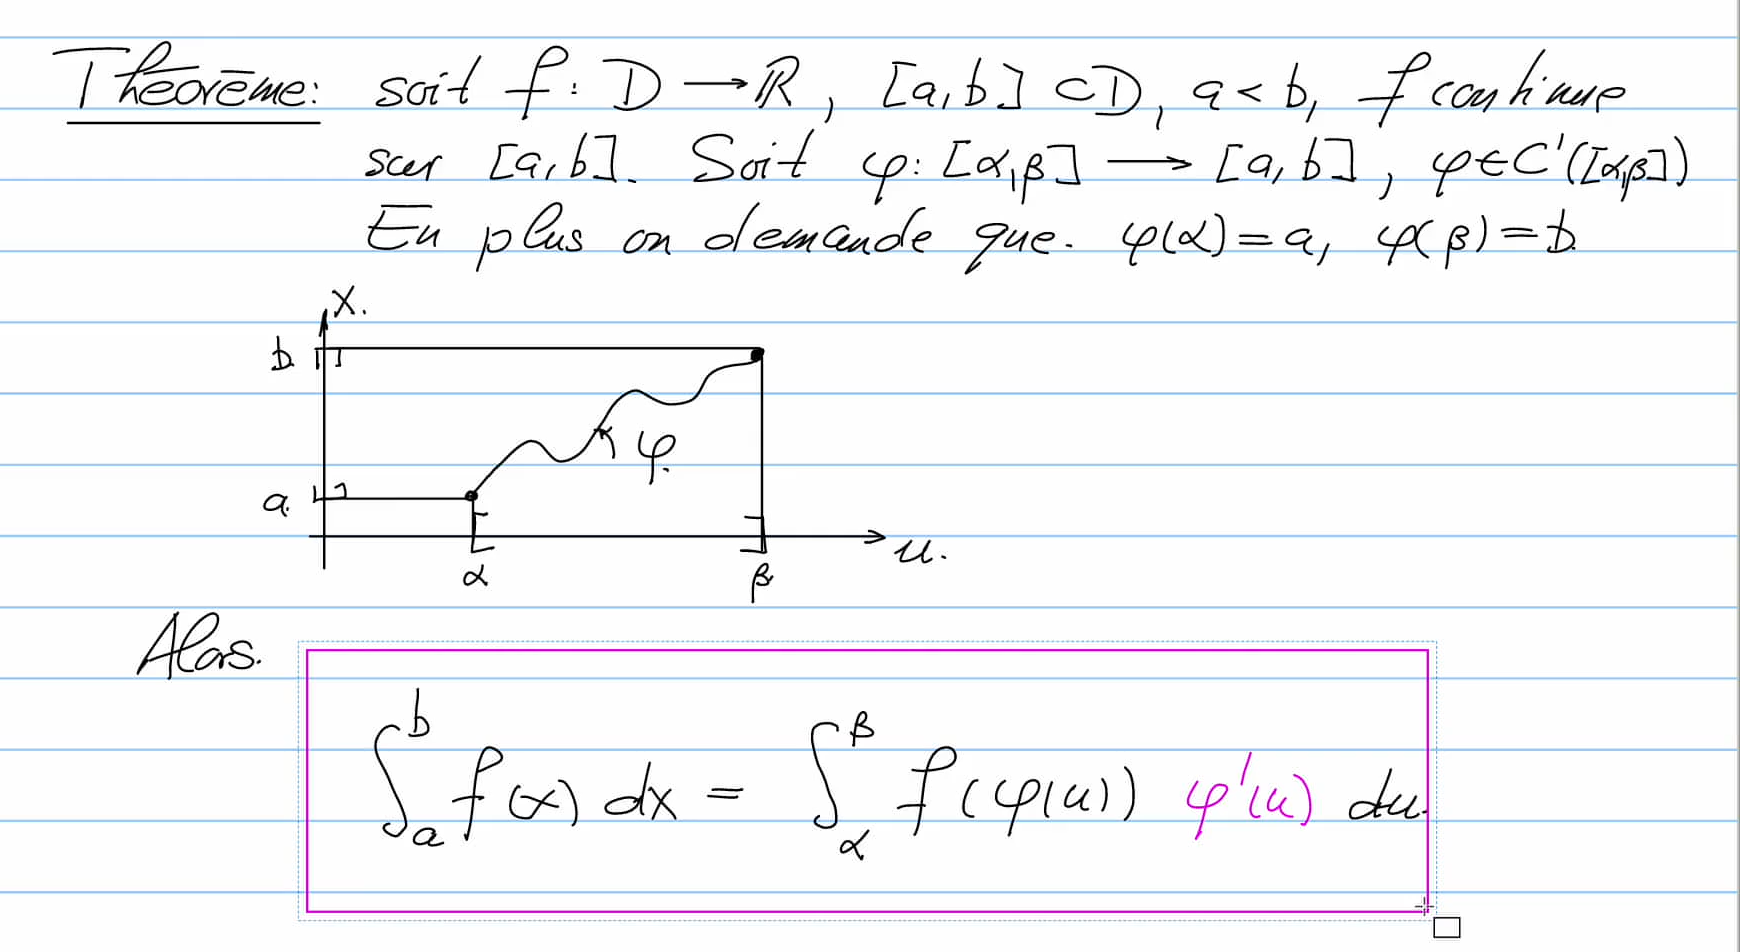
\includegraphics[width=1\linewidth]{image.png}
    \caption{Intégration par changement de variable}
    \label{fig:enter-label}
\end{figure}

\subsection{Intégration par partie}

voir image.

\begin{figure}
    \centering
    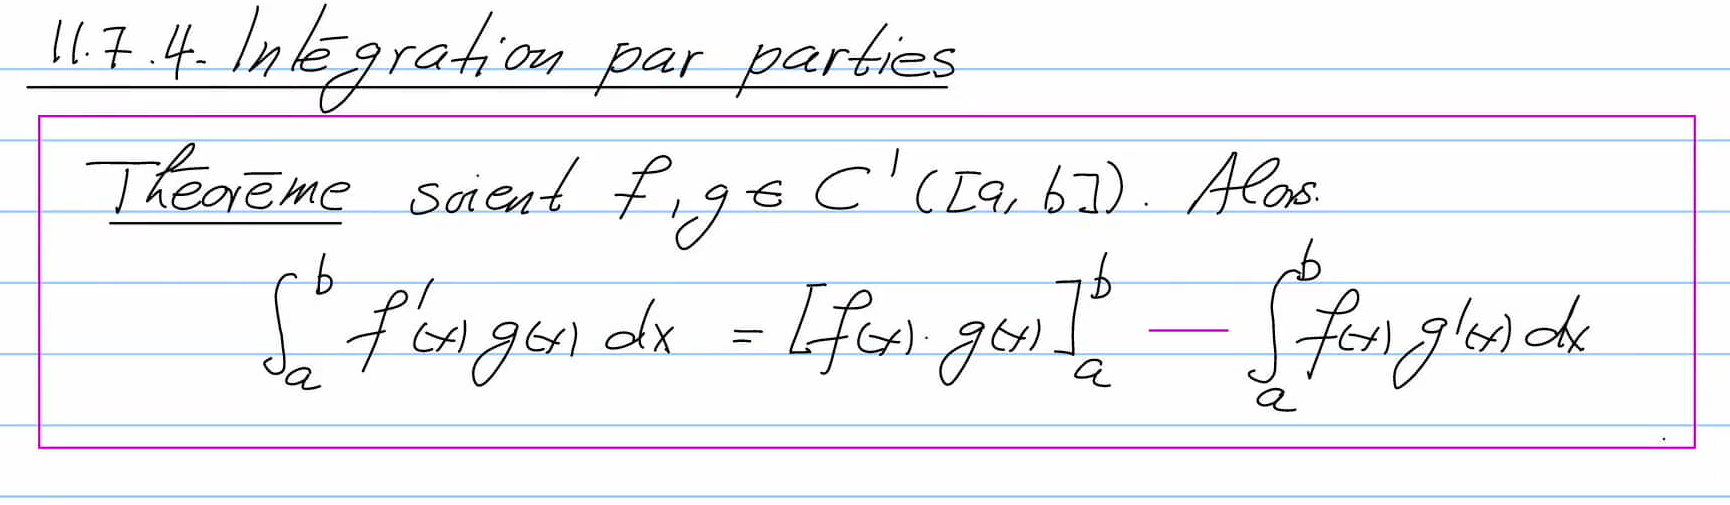
\includegraphics[width=1\linewidth]{partie.png}
    \caption{Enter Caption}
    \label{fig:enter-label}
\end{figure}

\subsection{Intégration par récurrence}

on cherche à exprimer $ I_{n+1} $ en fonction de $ I_n $.

\subsection{Intégrales impropres}

\subsubsection{Sous-Type 1}

$ f $ est continue sur $ [a,b[, ]a, b]$ ou $ ]a, b[ $.
\[ \int_{a}^{b-}f(x)dx = \lim_{\beta \to {b-}} \int_{a}^{\beta}f(x)dx \]
$ a < \beta < b $

\subsubsection{Sous-Type 2}

$ f $ continue sur $ ]-\infty, b], ]a, +\infty[, ]-\infty, +\infty[ $.
\[ \int_{-\infty}^{b}f(x)dx = \lim_{R \to {-\infty}} \int_{R}^{b}f(x)dx \]
b > R

\subsubsection{Sous-Type 3}

Combinaison des deux.
\[ \int_{-\infty}^{b-}f(x)dx = \lim_{{\beta \to {b-}}{R \to {-\infty}}} \int_{R}^{b}f(x)dx \]
$b > \beta > R > -\infty$ 

\end{document}
